\tikzset{every picture/.style={line width=0.75pt}} %set default line width to 0.75pt        

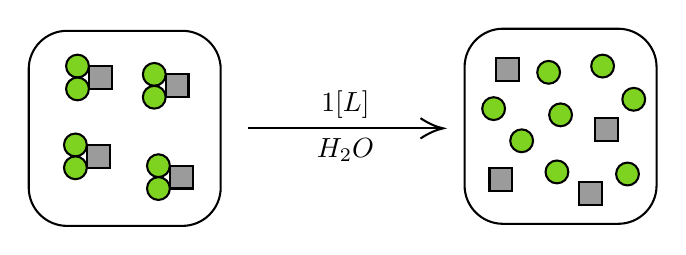
\begin{tikzpicture}[x=0.75pt,y=0.75pt,yscale=-1,xscale=1]
%uncomment if require: \path (0,300); %set diagram left start at 0, and has height of 300

%Rounded Rect [id:dp09558805847731922] 
\draw   (100,76.5) .. controls (100,66.28) and (108.28,58) .. (118.5,58) -- (174,58) .. controls (184.22,58) and (192.5,66.28) .. (192.5,76.5) -- (192.5,133.5) .. controls (192.5,143.72) and (184.22,152) .. (174,152) -- (118.5,152) .. controls (108.28,152) and (100,143.72) .. (100,133.5) -- cycle ;
%Shape: Square [id:dp7746522111111718] 
\draw  [fill={rgb, 255:red, 155; green, 155; blue, 155 }  ,fill opacity=1 ] (129,75) -- (140,75) -- (140,86) -- (129,86) -- cycle ;
%Shape: Circle [id:dp8391230190802568] 
\draw  [fill={rgb, 255:red, 126; green, 211; blue, 33 }  ,fill opacity=1 ] (118,75) .. controls (118,71.96) and (120.46,69.5) .. (123.5,69.5) .. controls (126.54,69.5) and (129,71.96) .. (129,75) .. controls (129,78.04) and (126.54,80.5) .. (123.5,80.5) .. controls (120.46,80.5) and (118,78.04) .. (118,75) -- cycle ;
%Shape: Circle [id:dp4898809706637761] 
\draw  [fill={rgb, 255:red, 126; green, 211; blue, 33 }  ,fill opacity=1 ] (118,86) .. controls (118,82.96) and (120.46,80.5) .. (123.5,80.5) .. controls (126.54,80.5) and (129,82.96) .. (129,86) .. controls (129,89.04) and (126.54,91.5) .. (123.5,91.5) .. controls (120.46,91.5) and (118,89.04) .. (118,86) -- cycle ;

%Shape: Square [id:dp737781660301758] 
\draw  [fill={rgb, 255:red, 155; green, 155; blue, 155 }  ,fill opacity=1 ] (128,113) -- (139,113) -- (139,124) -- (128,124) -- cycle ;
%Shape: Circle [id:dp5065662913612368] 
\draw  [fill={rgb, 255:red, 126; green, 211; blue, 33 }  ,fill opacity=1 ] (117,113) .. controls (117,109.96) and (119.46,107.5) .. (122.5,107.5) .. controls (125.54,107.5) and (128,109.96) .. (128,113) .. controls (128,116.04) and (125.54,118.5) .. (122.5,118.5) .. controls (119.46,118.5) and (117,116.04) .. (117,113) -- cycle ;
%Shape: Circle [id:dp4892788232253358] 
\draw  [fill={rgb, 255:red, 126; green, 211; blue, 33 }  ,fill opacity=1 ] (117,124) .. controls (117,120.96) and (119.46,118.5) .. (122.5,118.5) .. controls (125.54,118.5) and (128,120.96) .. (128,124) .. controls (128,127.04) and (125.54,129.5) .. (122.5,129.5) .. controls (119.46,129.5) and (117,127.04) .. (117,124) -- cycle ;

%Shape: Square [id:dp9750827491698186] 
\draw  [fill={rgb, 255:red, 155; green, 155; blue, 155 }  ,fill opacity=1 ] (166,79) -- (177,79) -- (177,90) -- (166,90) -- cycle ;
%Shape: Circle [id:dp26908352554943327] 
\draw  [fill={rgb, 255:red, 126; green, 211; blue, 33 }  ,fill opacity=1 ] (155,79) .. controls (155,75.96) and (157.46,73.5) .. (160.5,73.5) .. controls (163.54,73.5) and (166,75.96) .. (166,79) .. controls (166,82.04) and (163.54,84.5) .. (160.5,84.5) .. controls (157.46,84.5) and (155,82.04) .. (155,79) -- cycle ;
%Shape: Circle [id:dp9383530976667467] 
\draw  [fill={rgb, 255:red, 126; green, 211; blue, 33 }  ,fill opacity=1 ] (155,90) .. controls (155,86.96) and (157.46,84.5) .. (160.5,84.5) .. controls (163.54,84.5) and (166,86.96) .. (166,90) .. controls (166,93.04) and (163.54,95.5) .. (160.5,95.5) .. controls (157.46,95.5) and (155,93.04) .. (155,90) -- cycle ;

%Shape: Square [id:dp26635299800514867] 
\draw  [fill={rgb, 255:red, 155; green, 155; blue, 155 }  ,fill opacity=1 ] (168,123) -- (179,123) -- (179,134) -- (168,134) -- cycle ;
%Shape: Circle [id:dp13000172095781903] 
\draw  [fill={rgb, 255:red, 126; green, 211; blue, 33 }  ,fill opacity=1 ] (157,123) .. controls (157,119.96) and (159.46,117.5) .. (162.5,117.5) .. controls (165.54,117.5) and (168,119.96) .. (168,123) .. controls (168,126.04) and (165.54,128.5) .. (162.5,128.5) .. controls (159.46,128.5) and (157,126.04) .. (157,123) -- cycle ;
%Shape: Circle [id:dp9381753901326322] 
\draw  [fill={rgb, 255:red, 126; green, 211; blue, 33 }  ,fill opacity=1 ] (157,134) .. controls (157,130.96) and (159.46,128.5) .. (162.5,128.5) .. controls (165.54,128.5) and (168,130.96) .. (168,134) .. controls (168,137.04) and (165.54,139.5) .. (162.5,139.5) .. controls (159.46,139.5) and (157,137.04) .. (157,134) -- cycle ;

%Straight Lines [id:da48576334145945643] 
\draw    (297.67,105) -- (205.5,105) ;
\draw [shift={(299.67,105)}, rotate = 180] [color={rgb, 255:red, 0; green, 0; blue, 0 }  ][line width=0.75]    (10.93,-4.9) .. controls (6.95,-2.3) and (3.31,-0.67) .. (0,0) .. controls (3.31,0.67) and (6.95,2.3) .. (10.93,4.9)   ;
%Rounded Rect [id:dp5654289542883939] 
\draw   (310,75.5) .. controls (310,65.28) and (318.28,57) .. (328.5,57) -- (384,57) .. controls (394.22,57) and (402.5,65.28) .. (402.5,75.5) -- (402.5,132.5) .. controls (402.5,142.72) and (394.22,151) .. (384,151) -- (328.5,151) .. controls (318.28,151) and (310,142.72) .. (310,132.5) -- cycle ;
%Shape: Square [id:dp6851302359611957] 
\draw  [fill={rgb, 255:red, 155; green, 155; blue, 155 }  ,fill opacity=1 ] (373,100) -- (384,100) -- (384,111) -- (373,111) -- cycle ;
%Shape: Circle [id:dp546261540900238] 
\draw  [fill={rgb, 255:red, 126; green, 211; blue, 33 }  ,fill opacity=1 ] (345,78) .. controls (345,74.96) and (347.46,72.5) .. (350.5,72.5) .. controls (353.54,72.5) and (356,74.96) .. (356,78) .. controls (356,81.04) and (353.54,83.5) .. (350.5,83.5) .. controls (347.46,83.5) and (345,81.04) .. (345,78) -- cycle ;
%Shape: Circle [id:dp44562200766655] 
\draw  [fill={rgb, 255:red, 126; green, 211; blue, 33 }  ,fill opacity=1 ] (332,111) .. controls (332,107.96) and (334.46,105.5) .. (337.5,105.5) .. controls (340.54,105.5) and (343,107.96) .. (343,111) .. controls (343,114.04) and (340.54,116.5) .. (337.5,116.5) .. controls (334.46,116.5) and (332,114.04) .. (332,111) -- cycle ;
%Shape: Square [id:dp5597699275826751] 
\draw  [fill={rgb, 255:red, 155; green, 155; blue, 155 }  ,fill opacity=1 ] (325,71) -- (336,71) -- (336,82) -- (325,82) -- cycle ;
%Shape: Circle [id:dp5939049052624168] 
\draw  [fill={rgb, 255:red, 126; green, 211; blue, 33 }  ,fill opacity=1 ] (371,75) .. controls (371,71.96) and (373.46,69.5) .. (376.5,69.5) .. controls (379.54,69.5) and (382,71.96) .. (382,75) .. controls (382,78.04) and (379.54,80.5) .. (376.5,80.5) .. controls (373.46,80.5) and (371,78.04) .. (371,75) -- cycle ;
%Shape: Circle [id:dp6309506552111297] 
\draw  [fill={rgb, 255:red, 126; green, 211; blue, 33 }  ,fill opacity=1 ] (349,126) .. controls (349,122.96) and (351.46,120.5) .. (354.5,120.5) .. controls (357.54,120.5) and (360,122.96) .. (360,126) .. controls (360,129.04) and (357.54,131.5) .. (354.5,131.5) .. controls (351.46,131.5) and (349,129.04) .. (349,126) -- cycle ;
%Shape: Square [id:dp9427724360143306] 
\draw  [fill={rgb, 255:red, 155; green, 155; blue, 155 }  ,fill opacity=1 ] (322,124) -- (333,124) -- (333,135) -- (322,135) -- cycle ;
%Shape: Circle [id:dp13157535656505837] 
\draw  [fill={rgb, 255:red, 126; green, 211; blue, 33 }  ,fill opacity=1 ] (350.75,98.5) .. controls (350.75,95.46) and (353.21,93) .. (356.25,93) .. controls (359.29,93) and (361.75,95.46) .. (361.75,98.5) .. controls (361.75,101.54) and (359.29,104) .. (356.25,104) .. controls (353.21,104) and (350.75,101.54) .. (350.75,98.5) -- cycle ;
%Shape: Circle [id:dp04915295372897188] 
\draw  [fill={rgb, 255:red, 126; green, 211; blue, 33 }  ,fill opacity=1 ] (383,127) .. controls (383,123.96) and (385.46,121.5) .. (388.5,121.5) .. controls (391.54,121.5) and (394,123.96) .. (394,127) .. controls (394,130.04) and (391.54,132.5) .. (388.5,132.5) .. controls (385.46,132.5) and (383,130.04) .. (383,127) -- cycle ;
%Shape: Square [id:dp987165186169874] 
\draw  [fill={rgb, 255:red, 155; green, 155; blue, 155 }  ,fill opacity=1 ] (365,131) -- (376,131) -- (376,142) -- (365,142) -- cycle ;
%Shape: Circle [id:dp10313538325198679] 
\draw  [fill={rgb, 255:red, 126; green, 211; blue, 33 }  ,fill opacity=1 ] (386,91) .. controls (386,87.96) and (388.46,85.5) .. (391.5,85.5) .. controls (394.54,85.5) and (397,87.96) .. (397,91) .. controls (397,94.04) and (394.54,96.5) .. (391.5,96.5) .. controls (388.46,96.5) and (386,94.04) .. (386,91) -- cycle ;
%Shape: Circle [id:dp36049934969937447] 
\draw  [fill={rgb, 255:red, 126; green, 211; blue, 33 }  ,fill opacity=1 ] (318.5,95.5) .. controls (318.5,92.46) and (320.96,90) .. (324,90) .. controls (327.04,90) and (329.5,92.46) .. (329.5,95.5) .. controls (329.5,98.54) and (327.04,101) .. (324,101) .. controls (320.96,101) and (318.5,98.54) .. (318.5,95.5) -- cycle ;

% Text Node
\draw (252.59,101.6) node [anchor=south] [inner sep=0.75pt]    {$1[ L]$};
% Text Node
\draw (252.59,108.4) node [anchor=north] [inner sep=0.75pt]    {$H_{2} O$};


\end{tikzpicture}
